\documentclass[conference]{IEEEtran}
\IEEEoverridecommandlockouts
\usepackage{cite}
\usepackage{amsmath,amssymb,amsfonts}
\usepackage{graphicx}
\usepackage{textcomp}
\usepackage{xcolor}
\usepackage{booktabs}
\usepackage{url}
\def\BibTeX{{\rm B\kern-.05em{\sc i\kern-.025em b}\kern-.08em
    T\kern-.1667em\lower.7ex\hbox{E}\kern-.125emX}}
\setcounter{dbltopnumber}{3}
\renewcommand{\dbltopfraction}{0.95}
\renewcommand{\textfraction}{0.05}
\renewcommand{\floatpagefraction}{0.85}
\begin{document}

\title{Multi-View VLM Verification for Semantic Object Extraction from a
Terrestrial Laser Scan Toward TOSM-Based Robot Environment Models}

\author{\IEEEauthorblockN{Sangmin Kim$^{1,2}$,
Haryeong Kim$^{1}$,
Yonghyeon Song$^{1,2}$, and
Tae-Yong Kuc$^{1,2,*}$\thanks{$^{*}$Corresponding author: Tae-Yong Kuc (tykuc@skku.edu).}}
\IEEEauthorblockA{$^{1}$Dept.\ of Electrical and Computer Engineering, Sungkyunkwan University, Suwon 16419, Republic of Korea\\
$^{2}$CASELab Co., Ltd., Anyang 14118, Republic of Korea\\
kimsang.m@g.skku.edu, khy0403@skku.edu, songyong2535@g.skku.edu, tykuc@skku.edu}
}

\maketitle

\begin{abstract}
Semantic environment models such as the Triplet Ontological Semantic Model
(TOSM) give indoor mobile robots the symbolic, explicit, and implicit
knowledge needed for task-level autonomy, but populating them for an
existing facility is still manual work. This paper presents an automated
pipeline that extracts TOSM semantic objects from a single terrestrial
laser scan and emits them as a VDA~5050-style JSON message. A deterministic
stage segments the colored point cloud and fills the explicit model (pose,
dimensions, color) with a provisional class from an open-vocabulary 3D
classifier; a vision--language model (VLM) stage then verifies each class
from multi-view object renders under forced tool-use and infers the
implicit affordance model. We show that the obvious multi-view strategy ---
feeding all views into one prompt (early fusion) --- \emph{degrades}
accuracy on sparse point renders, and propose per-view classification with
confidence-weighted voting (late fusion) instead. On a 68.5M-point scan of
a robot showroom (57 objects), graded both by a render-based audit and by
an independent on-site inventory, late fusion is the strongest multi-view
strategy (74\% vs.\ 67\% lenient accuracy over early fusion), although a
single canonical view remains the most accurate configuration overall. The
robust benefit of the multi-view stage is a free reliability signal: label
votes unanimous across views are 94--95\% correct against the inventory in
three independent runs, versus 30\% for split votes --- gating validated
when the inventory overturned labels that had fooled both the VLM and the
human audit. Full-scene verification costs \$2.6; all prompts, settings,
and audits are released for reproduction.
\end{abstract}

\begin{IEEEkeywords}
multi-view object recognition, vision--language model, semantic mapping,
terrestrial laser scanning, TOSM, VDA 5050
\end{IEEEkeywords}

\section{Introduction}
Task-level autonomy for indoor mobile robots requires more than an
occupancy grid: the robot must know \emph{what} objects occupy the space,
\emph{where} they are, and \emph{how} they can be interacted with. The
Triplet Ontological Semantic Model (TOSM)~\cite{joo2020tosm} organizes this
knowledge into a \emph{symbolic} model (class, name, identity), an
\emph{explicit} model (pose, size, color), and an \emph{implicit} model
(affordances such as whether an object is a reliable landmark or can be
displaced). TOSM-style databases drive navigation frameworks and multi-robot
fleets, and their content maps naturally onto the JSON message conventions
of VDA~5050~\cite{vda5050}, the emerging interface standard between AGV
fleets and master control systems.

In practice, the semantic-object database for a new facility is authored by
hand. Terrestrial laser scanners (TLS) such as the Leica BLK360 capture a
dense, colored as-built model in minutes, and scan-to-BIM
research~\cite{patraucean2015} recovers structural geometry automatically,
but object-level semantics remain the gap: open-vocabulary 3D classifiers
such as Uni3D~\cite{zhou2024uni3d} are biased toward industrial structural
classes --- in our experiments office chairs were labeled \emph{stair} or
\emph{machine} and displays \emph{ladder} --- and no point-cloud classifier
produces the affordance-level knowledge TOSM needs.

Vision--language models (VLMs) offer a complementary signal: rendered views
of a segmented object carry texture and context that a point-cloud embedding
discards. Since multi-view recognition classically outperforms single-view,
we render each object from four azimuths and study how a VLM should consume
them. The naive strategy --- all views in one prompt (\emph{early fusion})
--- turns out to \emph{hurt}: sparse oblique point renders invite
over-confident misreadings that contaminate the joint judgment. Classifying
each view independently and aggregating by confidence-weighted vote
(\emph{late fusion}), the multi-view analogue of MVCNN-style
aggregation~\cite{su2015mvcnn}, recovers most of the lost reliability and
exposes disagreement between views as an explicit uncertainty signal. The contributions are:

\begin{itemize}
\item an automated TLS-to-TOSM pipeline whose output is a VDA~5050-style
      \texttt{semanticObjects} message consumable by a fleet environment
      model;
\item a schema-forced VLM verification protocol with per-view late fusion,
      plus prompt guardrails (size sanity, sparse-render caution, panel
      disambiguation) for point-render inputs;
\item a six-configuration study on a real 68.5M-point BLK360 scan (57
      objects), graded by a render-based audit and re-scored against an
      independent on-site inventory with repeat runs, showing that early
      fusion degrades accuracy, that late fusion is the strongest
      multi-view strategy while a single canonical view stays most
      accurate overall, and that vote unanimity yields 94--95\%-precise
      gating.
\end{itemize}

\begin{figure}[t]
\centering
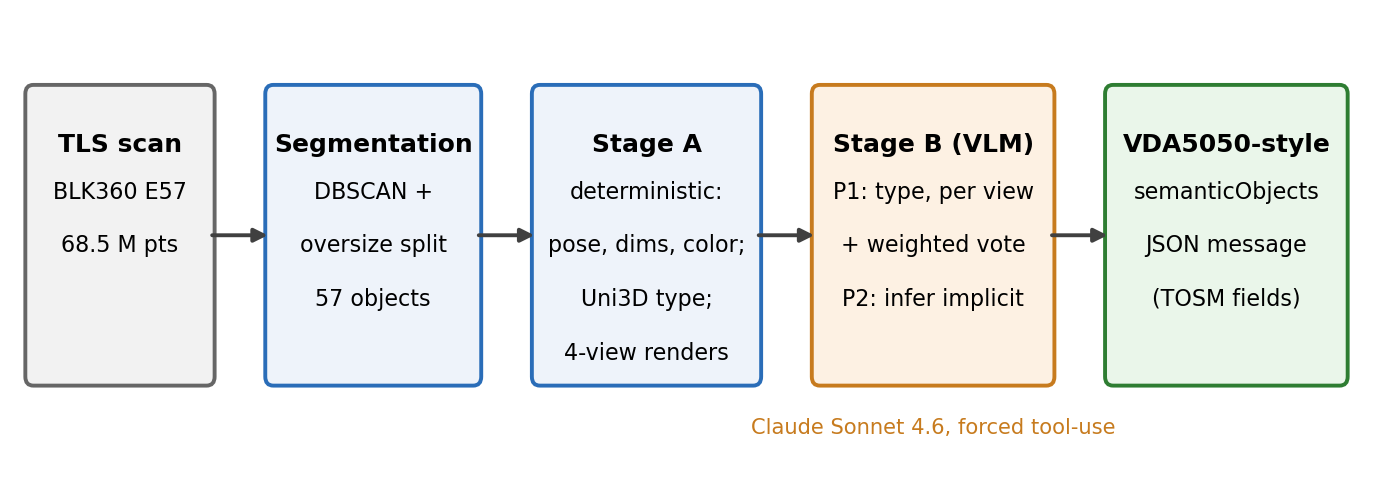
\includegraphics[width=0.86\columnwidth]{fig_pipeline.png}
\caption{Scan-to-semantics pipeline. Stage A deterministically fills the
explicit TOSM model plus a provisional class; Stage B (Claude Sonnet 4.6,
forced tool-use) verifies the symbolic model per view with weighted late
fusion and infers the implicit model.}
\label{fig:pipeline}
\end{figure}

\section{Related Work}
\textbf{Semantic environment models.} TOSM~\cite{joo2020tosm} extends
ontology-based robot knowledge bases~\cite{tenorth2013} with the
symbolic/explicit/implicit triplet; its records subsume the object fields of
VDA~5050~\cite{vda5050} messages, which we adopt as the output container;
the taxonomy also underpins a knowledge-grounded 3D scene graph for LLM
querying~\cite{kim2025isis}, whose records we populate automatically.
\textbf{Scan-to-model.} As-built modeling from TLS has focused on
structural elements~\cite{patraucean2015}; object semantics are left to
learned 3D segmentation~\cite{qi2017} or open-vocabulary encoders such as
Uni3D~\cite{zhou2024uni3d}, which inherit training-corpus biases.
\textbf{Multi-view recognition.} Aggregating rendered views is a classic
route to 3D shape recognition (MVCNN~\cite{su2015mvcnn}); we revisit the
early-vs-late fusion question for VLM prompts over \emph{sparse point}
renders rather than mesh renders. \textbf{VLMs in robotics.} Recent systems
use VLMs for open-set scene graphs~\cite{gu2024conceptgraphs} and
language-driven maps~\cite{huang2023vlmaps}. We use a VLM in a narrower,
auditable role: verifying one object at a time against measured geometry.

\section{Pipeline}

\subsection{Stage A: Deterministic Explicit Model}
\label{sec:stagea}
The input is a single registered BLK360 scan (E57, colored), voxel-
downsampled at 3\,cm. Structural planes are removed by a seeded RANSAC
(300 random triples per plane, 5\,cm inlier threshold, one SVD refit;
a plane is removed only if near-horizontal, $|n_z|\ge0.85$, or
near-vertical, $|n_z|\le0.2$; the loop stops after ten planes, when fewer
than 2{,}000 points remain, or when the best plane supports $<$4\% of the
remaining points or is slanted). Objects are then segmented by
DBSCAN~\cite{ester1996} with $\varepsilon=0.30$\,m and
$\mathrm{minPts}=100$, which yields 30 clusters on our scene; a
conservative re-clustering pass re-runs DBSCAN with
$\varepsilon=0.20$\,m inside every cluster whose footprint exceeds
2.5\,m, accepting the split only if it produces at least two sub-clusters
of $\ge$100 points, and raises the count to the 57 objects evaluated in
Sec.~\ref{sec:setup}; no further filtering was applied to the evaluated
set. Segmentation stays
geometric because ScanNet-trained instance segmenters did not transfer to
this industrial scene: on the same cloud, SPFormer assigned only 51\% of
points with furniture-biased labels, and PTv3 labeled 46\% of points
\emph{wall} even after wall removal. For each object Stage~A
computes the explicit TOSM model directly from the points: bounding-box
center (\texttt{poseX/Y}, \texttt{properties.poseZ}), PCA-based yaw
(\texttt{poseTheta}), yaw-aligned extents (\texttt{dimensions}), and a mean
RGB color name. Uni3D provides a \emph{provisional} symbolic class, and four
azimuth renders (0/90/180/270$^{\circ}$, elevation 25$^{\circ}$,
512$\times$512, point size~8, red 3D bounding box) are exported; smaller
point sizes produced speckle-like views that misled both the VLM and the
human auditors (Sec.~\ref{sec:study}). All Stage-A fields are measured,
not generated; Stage~B never modifies them.

\subsection{Stage B: VLM Verification with Late Fusion}
\label{sec:stageb}
Stage B calls a commercial VLM (Claude Sonnet 4.6, API model
\texttt{claude-sonnet-4-6}, 512 output tokens, default sampling
temperature) with \emph{forced tool-use}: the model must answer by calling
a declared JSON tool, so every response is schema-valid by construction.
Fig.~\ref{fig:prompt} condenses the prompt design; the full system prompts,
tool schemas, and configuration files are released with the
code\footnote{\url{https://github.com/kkk3449/tls-smf}}.

\emph{Prompt 1 (symbolic), once per view.} The VLM sees ONE render, the
measured dimensions, the provisional class, and an optional candidate
vocabulary. Candidates are not generated per object: the operator supplies
one scene-level list (\emph{chair, TV, monitor, Mobile Robot, desk} for
this scene), which is passed unchanged to every call. The decision
rule is three-way: keep a correct label; if wrong, prefer a fitting
candidate; else emit an open-vocabulary label. Guardrails address
point-render failure modes (Fig.~\ref{fig:prompt}): dimensions as a hard
constraint, oversize clusters treated as merged objects, thin-panel
disambiguation, a ban on claiming parts not outlined by points, and a
keep-or-\emph{clutter} fallback when no label is clearly supported.

\emph{Late fusion.} The four per-view reports are aggregated by
confidence-weighted voting: each label $\ell$ accumulates the confidences
of the views that voted for it, $s(\ell)=\sum_{v:\,\ell_v=\ell} c_v$; the
top-scoring label wins, and the final confidence is its share
$s(\ell^\star)/\sum_\ell s(\ell)$. The per-view votes are stored in the
record (\texttt{properties.viewVotes}), so a downstream consumer can
distinguish a 4/4 unanimous label from a 2/4 split --- an uncertainty
signal that costs nothing extra. Fig.~\ref{fig:votes} shows a unanimous
case: all four azimuths of a robot manipulator agree independently, giving
fused confidence 1.0. Conversely, a single contaminated view is simply
outvoted (a tall-backed chair whose frontal view read \emph{Mobile Robot}
fused to \emph{chair} 3:1), whereas the same view inside one early-fusion
prompt can drag the joint judgment toward the wrong label.

\begin{figure}[t]
\centering
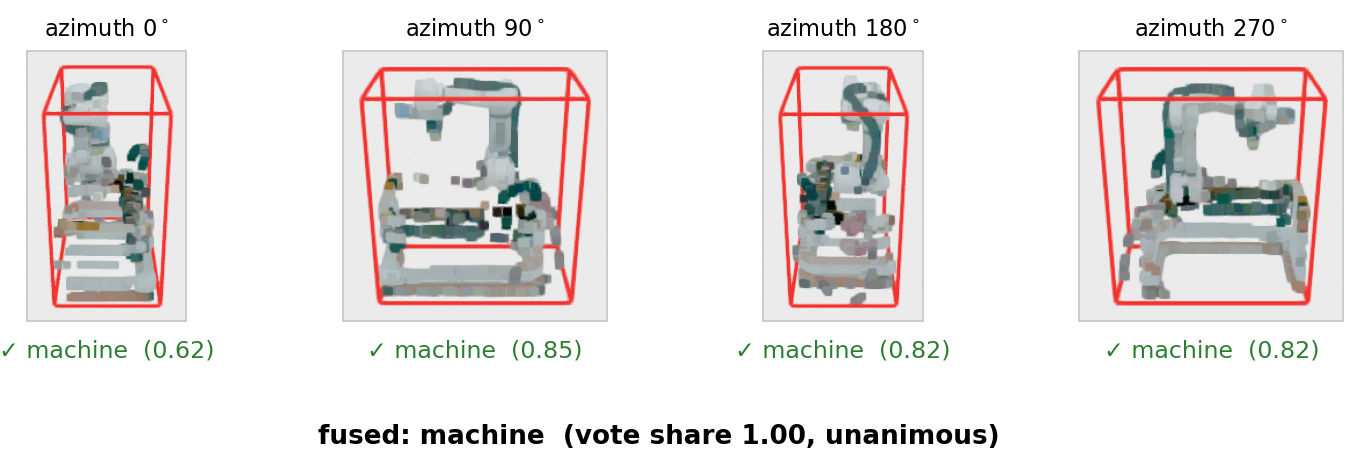
\includegraphics[width=0.74\columnwidth]{fig_votes.png}
\caption{Late fusion on one object (\texttt{machine\_004}). Each of the
four azimuth renders is classified independently; here all views agree,
yielding the unanimous, confidence-1.0 case that both the render audit and
the inventory find 94--95\% reliable (Sec.~\ref{sec:study}).}
\label{fig:votes}
\end{figure}

\emph{Prompt 2 (implicit), once per object.} Given the fused type and all
views, the VLM reports the TOSM implicit model: \texttt{isKeyObject},
\texttt{isMovable}, and (doors only) \texttt{isOpen}/\texttt{canBeOpen}.

\begin{figure}[t]
\centering
\fbox{\begin{minipage}{0.94\columnwidth}\footnotesize
\textbf{P1 system (condensed).} You are a semantic-mapping verifier for an
indoor mobile robot. You see a render of ONE segmented 3D object (sparse
laser points, red 3D box), its classifier label \texttt{uni3d\_type}, and
optional candidates. \emph{Decision rule:} (1)~if \texttt{uni3d\_type} is
correct, KEEP; (2)~if wrong, replace --- (a)~prefer a fitting candidate,
(b)~else the most accurate common-noun label. Never `unknown'.
\emph{Size sanity:} measured dimensions are a HARD constraint; a cluster
exceeding a class's envelope is merged objects --- label the dominant
structure or `clutter'. \emph{Sparse-render caution:} never claim parts not
clearly outlined by points. \emph{Panel rule:} thin flat objects are
keyboard (key grid) / display (uniform dark face) / shelf --- never ladder.
\emph{Chair gate:} requires visible seat pan 0.3--0.6\,m high plus
backrest. If uncertain, keep a size-compatible label. Respond ONLY via the
\texttt{report\_symbolic} tool.\\[2pt]
\textbf{P2 system (condensed).} Infer implicit properties of ONE object
from its views and confirmed type: \texttt{isKeyObject} (fixed, distinctive
landmark), \texttt{isMovable}, \texttt{isOpen}/\texttt{canBeOpen} (doors
only, else null). Respond ONLY via the \texttt{report\_implicit} tool.
\end{minipage}}
\caption{Condensed Stage-B prompt design (full text in the released code).
Forced tool-use makes every response schema-valid JSON; measured geometry
is read-only context.}
\label{fig:prompt}
\end{figure}

\subsection{TOSM to VDA 5050-Style Message}
The completed records are serialized as one \texttt{semanticObjects} JSON
message with a VDA~5050-style header. Table~\ref{tab:mapping} shows the
field mapping; TOSM fields with no standard slot travel in the extensible
\texttt{properties} map, so the message remains readable by consumers that
only know the base schema.

\begin{table}[t]
\caption{TOSM $\rightarrow$ VDA 5050-style JSON field mapping}
\label{tab:mapping}
\centering
\scriptsize
\begin{tabular}{@{}lll@{}}
\toprule
TOSM model & element & JSON field \\
\midrule
symbolic & class & \texttt{type} \\
         & name / identity & \texttt{name}, \texttt{id} \\
explicit & position $(x,y)$ & \texttt{poseX}, \texttt{poseY} \\
         & height $z$ & \texttt{properties.poseZ} \\
         & orientation & \texttt{poseTheta} \\
         & size & \texttt{dimensions\{l,w,h\}} \\
         & color & \texttt{color} \\
implicit & landmark / movability & \texttt{properties.isKeyObject,} \\
         & door state & \texttt{isMovable, isOpen, canBeOpen} \\
--       & VLM audit trail & \texttt{properties.viewVotes,} \\
         &                 & \texttt{symbolicReason, confidence} \\
\bottomrule
\end{tabular}
\end{table}

\section{Experiments}

\begin{figure*}[t]
\centering

\includegraphics[width=0.62\textwidth]{fig_accuracy.png}
\caption{Effect of VLM verification on the 57-object scene. (a)~Class
distribution, classifier-only vs.\ after late fusion: implausible
\emph{ladder}/\emph{stair} populations are redistributed to displays and
furniture (the keyboard outputs were later rejected by the on-site
inventory, Sec.~\ref{sec:study}). (b)~Render audit: early fusion degrades
single-view accuracy; late fusion is the strongest multi-view strategy (15
wrong labels vs.\ 19 for early fusion).}
\label{fig:accuracy}
\end{figure*}

\begin{figure*}[!t]
\centering
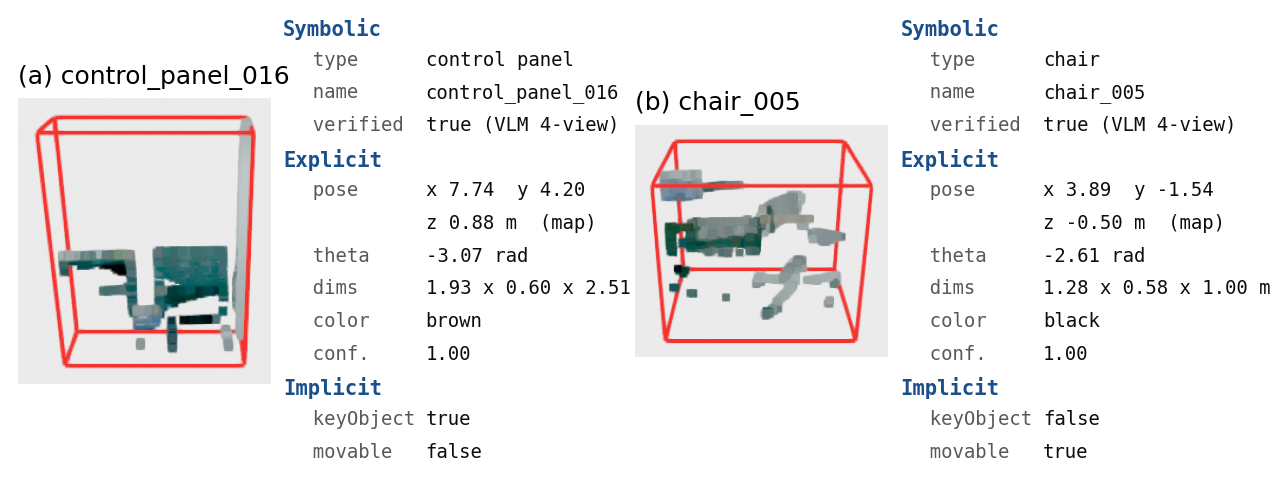
\includegraphics[width=0.62\textwidth]{fig_cards.png}
\caption{Completed TOSM semantic-object records (dense render + symbolic /
explicit / implicit fields) as serialized into the VDA 5050-style message.
(a)~A control panel, unanimously verified and marked as a fixed key
landmark. (b)~An office chair corrected from \emph{stair}, movable and not
a landmark.}
\label{fig:cards}
\end{figure*}


\subsection{Setup, Audit Protocol, and Reference Labels}
\label{sec:setup}
We evaluate on a single BLK360 scan of an indoor robot showroom (68.5M
colored points, 57 segmented objects) with Claude Sonnet 4.6. Six
configurations are compared (Table~\ref{tab:configs}). They form a
$2\times2$ design over view count (1 vs.\ 4, early fusion) and render/prompt
generation (initial sparse renders with the base prompt vs.\ dense renders
with the guardrail prompt), plus a sixth configuration that differs from
four-view early fusion (dense) \emph{only} in the fusion rule; the render
density and the guardrails were upgraded together and are therefore not
separable in this study, whereas the fusion contrast is isolated. Metered
cost: late fusion \$2.63 per scene (285 calls, \$0.046/object); early
fusion \$1.27; single view \$0.87.

Labels are graded by two independent references. (i)~\emph{Render audit:}
two of the authors audited all 57 objects against the \emph{dense}
four-view renders and the measured dimensions, rating every
configuration's final label \emph{correct}, \emph{plausible} (consistent
with the views but not verifiable from renders alone), or \emph{wrong}.
(ii)~\emph{On-site inventory:} the facility operator subsequently assigned
every object a ground-truth type by physical inspection of the room,
without reference to the render audit (43 confirmed, 12 plausible, 2
unknown; 7 clusters were identified as ceiling-soffit structure remnants).
Inventory scoring is strict --- a label counts only if it equals the
inventory type, so a conservative \emph{clutter} on a real chair is wrong
--- and is reported on all 57 objects and on the 36 confirmed non-structure
objects. Agreement between the two references (audit \emph{correct} vs.\
inventory match) is 79--95\% across the five VLM configurations (Cohen's
$\kappa$ 0.53--0.89; 89\%, $\kappa=0.79$ for late fusion), so the render
audit is a faithful but not perfect proxy: for late fusion the two
references agree on every object, and across all configurations the
audit's optimistic calls are confined to \emph{handrail} labels on
soffit remnants (an artifact of the render), while its single
pessimistic call concerns an object the inventory itself marks unknown.

\subsection{Multi-View Study}
\label{sec:study}
Table~\ref{tab:configs} and Fig.~\ref{fig:accuracy}(b) summarize the
audit. Three findings stand out.

\emph{(1) Early fusion hurts.} Feeding four sparse views into one prompt
dropped strict accuracy from 60\% (single view) to 49\%: extra oblique
speckle views encouraged over-committed readings, e.g.\ two electrical
cabinets confidently relabeled \emph{chair}. Denser renders and the prompt
guardrails did not close the gap (46\% vs.\ 51\%). The inventory confirms
the direction: four-view early fusion is the worst VLM configuration under
both references.

\emph{(2) Late fusion is the strongest multi-view strategy, but not the
best configuration.} Judging each view independently and voting beats
early fusion on every measure (15 vs.\ 19 wrong labels, 74\% vs.\ 67\%
lenient; 34 vs.\ 30 inventory matches): a contaminated view can no longer
dominate --- it is outvoted. It does not, however, overtake the best
single canonical view (60\%/81\% audit; 44 of 57 inventory matches, 77\%,
95\% Wilson CI 65--86\%, against 60\%, CI 47--71\% for late fusion): on
sparse point clouds, extra views add noise faster than evidence unless
aggregation is vote-based, and even then the vote spends much of its gain
on caution. The cost of voting is a larger \emph{plausible} bucket ---
split votes often land on \emph{clutter} --- which the strict inventory
counts as wrong and which is why late fusion's inventory score exceeds the
classifier's by only one object (34 vs.\ 33). We therefore claim
late fusion as the safer multi-view rule, not as an accuracy gain over a
well-chosen single view; the measurable value of the multi-view stage is
the reliability signal below.

\emph{(3) Vote unanimity is a free precision signal.} 17 of 57 objects
received identical labels from all four views; 16 of those (94\%) were
audited correct, and the same 16 match the inventory, versus 30\% (audit)
or 18/40 (inventory) among split-vote objects. Gating on the stored
\texttt{viewVotes} thus gives a downstream consumer a calibrated
route-to-human-review policy that per-call confidence alone did not
provide.

\emph{Repeatability.} Because the VLM samples stochastically, we re-ran
the late-fusion protocol twice more on the 50 non-structure objects at a
later date. Final labels agreed between the two re-runs on 82\% of
objects, and accuracy on the 36 confirmed objects was 28, 27, and 27 in
the three runs ($\pm$1 object); unanimity precision was 16/17, 20/21, and
19/20 (94--95\%) and split-vote accuracy 45\%, 28\%, and 30\%. The
ranking of configurations is thus stable to sampling, but the
single-scene, 57-object sample yields confidence intervals of roughly
$\pm$12 points, and all comparative claims are scoped to this scene.

Render density cut both ways, and produced the study's starkest warning:
dense renders made four dotted-grid panels look so convincingly like
keyboards (per-view confidence up to 0.97) that the label passed our
render-based audit --- only the inventory revealed them to be
ceiling-soffit remnants, and Table~\ref{tab:configs} grades every such
label wrong. The incident is the strongest argument for the gating above:
a label that fools both the VLM and a human at the same renders was still
caught by vote splits (these objects never reached unanimity); it also
motivated a structure-remnant filter that now removes such clusters in
Stage~A of our current pipeline.

\begin{table}[t]
\caption{Final type labels (57 objects) under both references. Render
audit: C/P/W = correct / plausible / wrong, strict = C, lenient = C+P.
Inventory: strict matches on all 57 objects and on the 36 confirmed
non-structure objects.}
\label{tab:configs}
\centering
\footnotesize
\setlength{\tabcolsep}{3.5pt}
\begin{tabular}{@{}lccccc|cc@{}}
\toprule
 & \multicolumn{5}{c|}{Render audit} & \multicolumn{2}{c}{Inventory} \\
Configuration & C & P & W & strict & lenient & 57 & 36 \\
\midrule
Uni3D only (no VLM)            & 28 & 5  & 24 & 49\% & 58\% & 33 & 28 \\
1 view, base prompt, sparse    & 34 & 12 & 11 & 60\% & 81\% & \textbf{44} & \textbf{33} \\
4 views early fus., sparse     & 28 & 10 & 19 & 49\% & 67\% & 34 & 27 \\
1 view, guardrails, dense      & 29 & 11 & 17 & 51\% & 70\% & 32 & 29 \\
4 views early fus., dense      & 26 & 12 & 19 & 46\% & 67\% & 30 & 23 \\
4 views late fus., dense & 28 & \textbf{14} & \textbf{15}
  & 49\% & \textbf{74\%} & 34 & 28 \\
\bottomrule
\end{tabular}
\end{table}

\begin{figure}[t]
\centering
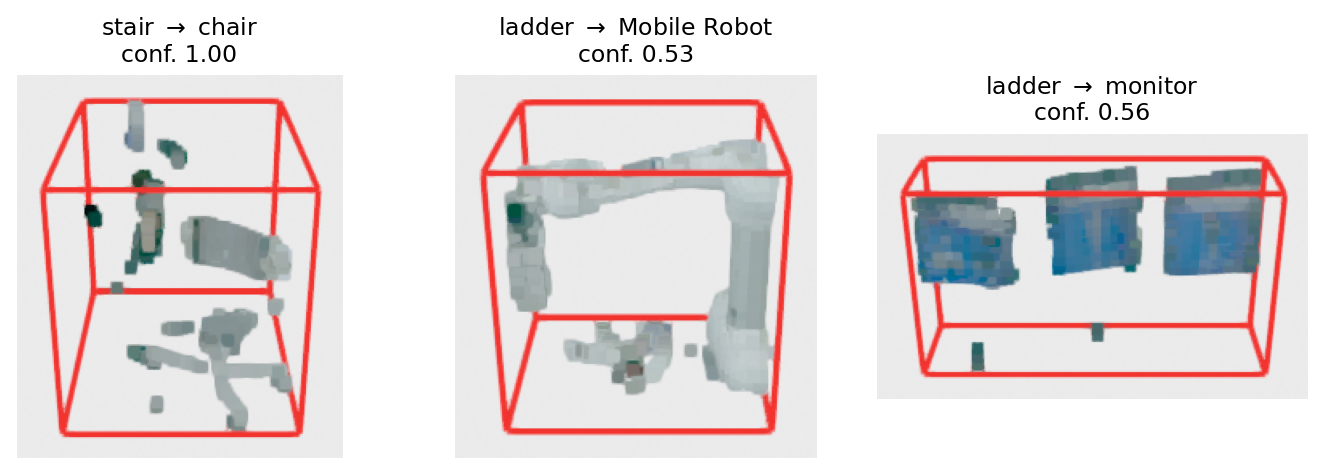
\includegraphics[width=0.58\columnwidth]{fig_examples.png}
\caption{Representative late-fusion corrections (one of four dense views;
provisional label $\rightarrow$ fused label, vote-share confidence). The 3D
classifier's industrial bias (\emph{stair}, \emph{ladder}) is corrected to
furniture, robots, and displays; a unanimous verification is detailed
view-by-view in Fig.~\ref{fig:votes}.}
\label{fig:examples}
\end{figure}



\subsection{Implicit Model and Completed Records}
On the late-fusion output, Prompt 2 marked 6 of 57 objects as key objects
(control panels, a large machine, mobile robots, a wall display) and 50 as
movable. Fig.~\ref{fig:cards} shows two completed TOSM records as stored in
the output message, including the audit trail (per-view votes, fused
confidence, one-sentence reason). Mean fused confidence was 0.71, and the
17 unanimous objects carry confidence 1.0 by construction, aligning the
stored confidence with the observed 94\% unanimity precision. By design
the generated records are a reviewable draft, not ground truth: the
semantic model remains user-editable and every amendment is logged in the
record's audit trail. An owner review exercised exactly this loop on the
implicit model, correcting two movability entries (a wheeled machine
judged fixed, a wall-mounted display judged movable) at negligible cost.

\subsection{Discussion and Limitations}
The division of labor is the main design point: everything measurable stays
deterministic and VLM-immutable, so hallucination can corrupt neither poses
nor dimensions, and the VLM contributes exactly the judgments geometry
cannot make --- naming and affordances --- in an auditable form (per-view
votes, forced-tool JSON, stored reasons). All 741 tool calls
across the five VLM configurations returned schema-valid
JSON. Remaining errors concentrate where the render itself is ambiguous
(texture-poor slabs, merged clusters, sparse strips), pointing to upstream
fixes --- finer segmentation, mesh renders --- not to the fusion protocol.
Absolute strict accuracy ($\sim$46--60\% audit, 53--77\% inventory)
reflects a deliberately hard test bed: a cluttered showroom scanned once,
without manual cleanup. The study's limits are its single scene and
57-object sample; the render-density and prompt factors are confounded;
and the inventory, while independent of the render audit, was compiled by
one operator. Multi-scene evaluation with per-factor ablation is future
work.

\section{Conclusion}
We presented an automated pipeline that turns a single terrestrial laser
scan into TOSM semantic-object records delivered as a VDA 5050-style JSON
message, using a VLM in a tightly scoped, schema-forced role. A
six-configuration study, graded by a render audit and an independent
on-site inventory, showed that the intuitive multi-view prompt --- all
views at once --- degrades verification on sparse point renders, whereas
per-view classification with confidence-weighted late fusion is the
strongest multi-view strategy (wrong labels 24$\rightarrow$15, 74\%
lenient accuracy), although a single canonical view remains the most
accurate configuration on this scene. The robust benefit of the
multi-view stage is its vote signal: unanimity provides a 94--95\%-precise
gate across three independent runs at \$2.6 per scene. Future work
includes mesh-based renders, finer segmentation, multi-scene evaluation,
and coupling the records to place modeling and a live digital twin.

\begin{thebibliography}{00}
\bibitem{joo2020tosm} S.-H. Joo \emph{et al.}, ``Autonomous navigation
framework for intelligent robots based on a semantic environment modeling,''
\emph{Applied Sciences}, vol.~10, no.~9, p.~3219, 2020.
\bibitem{vda5050} VDA and VDMA, ``VDA 5050: Interface for the communication
between automated guided vehicles (AGV) and a master control,'' ver.~2.0,
2022.
\bibitem{patraucean2015} V. P\u{a}tr\u{a}ucean, I. Armeni, M. Nahangi,
J. Yeung, I. Brilakis, and C. Haas, ``State of research in automatic
as-built modelling,'' \emph{Adv. Eng. Informat.}, vol.~29, no.~2,
pp.~162--171, 2015.
\bibitem{zhou2024uni3d} J. Zhou, J. Wang, B. Ma, Y.-S. Liu, T. Huang, and
X. Wang, ``Uni3D: Exploring unified 3D representation at scale,'' in
\emph{Proc. Int. Conf. Learn. Represent. (ICLR)}, 2024.
\bibitem{su2015mvcnn} H. Su, S. Maji, E. Kalogerakis, and E.
Learned-Miller, ``Multi-view convolutional neural networks for 3D shape
recognition,'' in \emph{Proc. IEEE Int. Conf. Comput. Vis. (ICCV)}, 2015,
pp.~945--953.
\bibitem{tenorth2013} M. Tenorth and M. Beetz, ``KnowRob: A knowledge
processing infrastructure for cognition-enabled robots,'' \emph{Int. J.
Robot. Res.}, vol.~32, no.~5, pp.~566--590, 2013.
\bibitem{kim2025isis} H. Kim, K. Joo, G. Galvis Giraldo, S. Kim, and
T.-Y. Kuc, ``Toward long-term memory in embodied AI: A knowledge-grounded
3D scene graph framework,'' in \emph{Proc. 26th Int. Symp. Adv. Intell.
Syst. (ISIS)}, Cheongju, Korea, 2025, pp. 237--240.
\bibitem{qi2017} C. R. Qi, H. Su, K. Mo, and L. J. Guibas, ``PointNet: Deep
learning on point sets for 3D classification and segmentation,'' in
\emph{Proc. IEEE Conf. Comput. Vis. Pattern Recognit. (CVPR)}, 2017,
pp.~652--660.
\bibitem{gu2024conceptgraphs} Q. Gu \emph{et al.}, ``ConceptGraphs:
Open-vocabulary 3D scene graphs for perception and planning,'' in
\emph{Proc. IEEE Int. Conf. Robot. Autom. (ICRA)}, 2024, pp.~5021--5028.
\bibitem{huang2023vlmaps} C. Huang, O. Mees, A. Zeng, and W. Burgard,
``Visual language maps for robot navigation,'' in \emph{Proc. IEEE Int.
Conf. Robot. Autom. (ICRA)}, 2023, pp.~10608--10615.
\bibitem{ester1996} M. Ester, H.-P. Kriegel, J. Sander, and X. Xu, ``A
density-based algorithm for discovering clusters in large spatial databases
with noise,'' in \emph{Proc. 2nd Int. Conf. Knowl. Discov. Data Min.
(KDD)}, 1996, pp. 226--231.
\end{thebibliography}

\end{document}
